%!TEX encoding = UTF-8 Unicode
%%% APSIPA 向け LaTeX テンプレート
\def\APSIPAyear{2017}
\ifdefined\pfmtname
   \documentclass[dvipdfmx,conference,a4paper,nofonttune]{APSIPA}
\else
   \documentclass[conference,a4paper,nofonttune]{APSIPA}
\fi
%!TEX encoding = UTF-8 Unicode
%
% 卒論 / 修論用 プリアンブル
%

%% フォント
\usepackage{lmodern}
\usepackage[scale=0.95]{tgheros}
\usepackage{textcomp}
\usepackage[scaled=0.85]{beramono}
\usepackage[T1]{fontenc}

%% パッケージ
\usepackage[cmex10]{amsmath}
\usepackage{amssymb,amsfonts,mathtools,bm}

\usepackage{graphicx,color}
\usepackage[table]{xcolor}

\usepackage[pdfborder={0 0 0}]{hyperref}
\usepackage{pxjahyper}

% caption のコロン「図4.4: キャプション」を「図4.4 キャプション」に直す
\usepackage[labelsep=quad,compatibility=false]{caption}
\usepackage[belowskip=1.2em]{subcaption}

\usepackage{cite,url,array,makecell}
\usepackage{algorithm,algorithmic}

% 数学コマンドの補完
\DeclareMathOperator*{\sinc}{sinc}
\DeclareMathOperator*{\prox}{prox}
\DeclareMathOperator*{\argmin}{argmin}
\DeclareMathOperator*{\argmax}{argmax}

% 参考文献表示スタイルを変更
\bibliographystyle{sieicej}

% 赤色を少し暗くする
\definecolor{red}{rgb}{0.75,0,0}

\makeatletter
   % アルゴリズム図キャプションの表記を「Algorithm」→「アルゴリズム」に
   \renewcommand{\ALG@name}{アルゴリズム}
\makeatother

% 修正箇所に色付けするコマンド
%
% ・ コマンド版
%   \fixed{修正箇所}
%
% ・ 環境版
%   \begin{fixedregion}
%      修正箇所
%   \end{fixedregion}
\newcommand{\fixed}[1]{#1} 
\newenvironment{fixedregion}{\ignorespaces}{\ignorespacesafterend}
% 下の 2 行をコメントアウトすることで色付けを無効化します
\renewcommand{\fixed}[1]{\textcolor{red}{#1}}
\renewenvironment{fixedregion}{\protect\leavevmode\color{red}\ignorespaces}{\ignorespacesafterend}

% 強調
\newcommand{\strong}[1]{\textcolor{red}{\textbf{#1}}}



%% \title : 一般の LaTeX 文書と同じ
%% 各単語の頭を大文字にする (前置詞とかを除いて)
\title{Guidelines for APSIPA ASC2017 Manuscripts}

%% \author : 以下の様に組む
%  +---------------------------+
%  |  \IEEEauthorblockN (名前)  |
%  +---------------------------+
%  |  \IEEEauthorblockA (所属)  |
%  +---------------------------+
\author{%
   \IEEEauthorblockN{Takanori Fujisawa, Masaaki Ikehara}
   \IEEEauthorblockA{EEE Dept., Keio Univ., Yokohama, Kanagawa 223-8522, Japan\\
   Email: \texttt{\url{{fujisawa,ikehara}@tkhm.elec.keio.ac.jp}}}
}

\begin{document}

\maketitle
\thispagestyle{empty}

\begin{abstract}
%% 概要
This document is an example of what your final camera-ready
manuscript to APSIPA ASC 2012 should look like.  Authors are asked
to conform to the directions reported in this document.
\end{abstract}

\section{General Instructions}

\subsection{Type Sizes and Typefaces}
Follow the type sizes specified in Table I.  As an aid in gauging type
size, 1 point is about 0.35 mm.  The size of the lowercase letter
``j'' will give the point size.  Times New Roman is the preferred
font.

\section{Helpful Hints}

\subsection{References}
Number citations consecutively in square brackets \cite{Eason1955}.  Punctuation
follows the bracket \cite{Maxwell1892}. Refer simply to the reference number, as in
\cite{Jacobs1963}. Use ``Ref. \cite{Jacobs1963}'' or ``Reference \cite{Jacobs1963}'' at the beginning of a
sentence: ``Reference \cite{Jacobs1963} was the first ...''


Gather the full set of references together in the section of
references.  Place the section of references before any appendices,
unless they contain references.  Arrange the references in
alphabetical order or in order of appearance in the paper.

Give all authors' names; use ``et al.''  if there are six authors or
more.  Papers that have not been published, even if they have been
submitted for publication, should be cited as ``unpublished'' \cite{Elissa}.
Papers that have been accepted for publication should be cited as ``in
press'' \cite{Nicole}.  In a paper title, capitalize the first word and all
other words except for conjunctions, prepositions less than seven
letters, and prepositional phrases.

For papers published in translated journals, first give the English
citation, then the original foreign-language citation \cite{Yorozu1987}.

% 引用は下のようにまとめて与えることができます
\cite{Eason1955,Maxwell1892,Jacobs1963,Elissa,Nicole,Yorozu1987,Young1989}


\subsection{Appendices}
Although conference papers do not normally have an appendix,
appendices, if any, directly follow the text and the references, (but
see IV.B).  Letter them in sequence and provide an informative title:
\textbf{Appendix A Title of Appendix}.

\subsection{Footnote}
Number footnotes separately in superscripts like this\footnote{This is
  how a footnote should appear.}.  Place the actual footnote at the
bottom of the column in which it was cited.  Footnotes should be
separated from the text by a line\footnote{Note the line separating
  the footnotes from the text.}.  Do not put footnotes in the
reference list. 


\subsection{Abbreviations and Acronyms}

Define abbreviations and acronyms the first time they are used in the
text, even if they have been defined in the abstract.  Abbreviations
such as APSIPA, SI, MKS, CGS, ac, dc, and rms do not have to be defined.
Do not use abbreviations in the title unless they are unavoidable.

\begin{table}[t]
   \centering
   \caption{Example of the multiple tables}
   \begin{minipage}{.45\hsize}
      \centering
      \subcaption{Table A}
      \begin{tabular}{|c|c|c|}
      \hline
       & & \\
      \hline
       & & \\
      \hline
      \end{tabular}
   \end{minipage}
   \begin{minipage}{.45\hsize}
      \centering
      \subcaption{Table B}
      \begin{tabular}{|c|c|c|}
      \hline
       & & \\
      \hline
       & & \\
      \hline
      \end{tabular}
   \end{minipage} \\[1.5em]
   \begin{minipage}{.45\hsize}
      \centering
      \subcaption{Table C}
      \begin{tabular}{|c|c|c|}
      \hline
       & & \\
      \hline
       & & \\
      \hline
      \end{tabular}
   \end{minipage}
   \begin{minipage}{.45\hsize}
      \centering
      \subcaption{Table D}
      \begin{tabular}{|c|c|c|}
      \hline
       & & \\
      \hline
       & & \\
      \hline
      \end{tabular}
   \end{minipage}
\end{table}

\begin{figure}[t]
   \centering
   \begin{minipage}{.45\hsize}
      \centering
      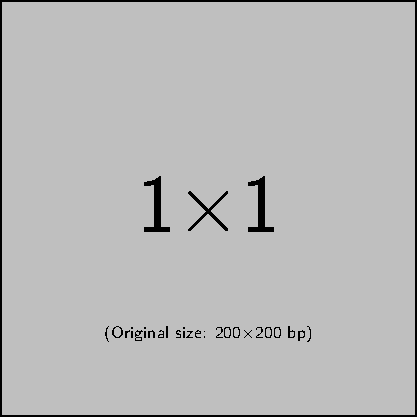
\includegraphics[width=.8\hsize]{figure/example-image-1x1.pdf}
      \subcaption{aaa}
   \end{minipage}
   \begin{minipage}{.45\hsize}
      \centering
      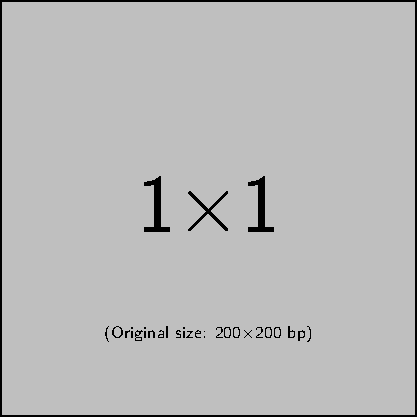
\includegraphics[width=.8\hsize]{figure/example-image-1x1.pdf}
      \subcaption{aaa}
   \end{minipage} \\[1em]
   \begin{minipage}{.45\hsize}
      \centering
      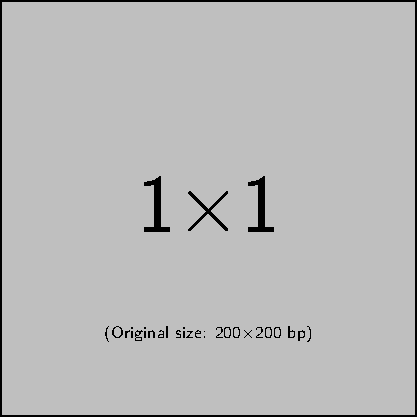
\includegraphics[width=.8\hsize]{figure/example-image-1x1.pdf}
      \subcaption{aaa}
   \end{minipage}
   \begin{minipage}{.45\hsize}
      \centering
      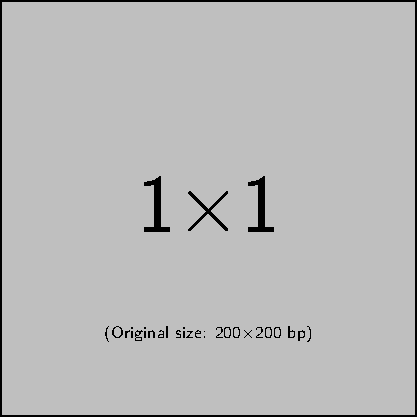
\includegraphics[width=.8\hsize]{figure/example-image-1x1.pdf}
      \subcaption{aaa}
   \end{minipage}
   \caption{Example of the figure placed in $2\times2$ layout.}
\end{figure}

\begin{table}[t]
   \centering
   \caption{Example of the table}
   \begin{tabular}{|c|p{40mm}|c|c|}
\hline
& \multicolumn{3}{c|}{Appearance}\\
\cline{2-4}
Size & \multicolumn{1}{c|}{Regular} & Bold & Italic \\
\hline
6 & Table captions, table subscripts & & \\
\cline{2-4}
8 & Section titles, references, tables, table names, first letters in table 
captions, figure captions, footnotes, text subscripts, and superscripts & & \\
\cline{2-4}
9 & & Abstract & \\
\cline{2-4}
10 & Authors, affiliations, main text, equations, first letters in section titles & & Subheading \\
\cline{2-4}
11 & Authors' names & & \\
\cline{2-4}
24 & Paper title   & & \\
\hline
   \end{tabular}
\end{table}

\begin{figure*}[t]
   \centering
   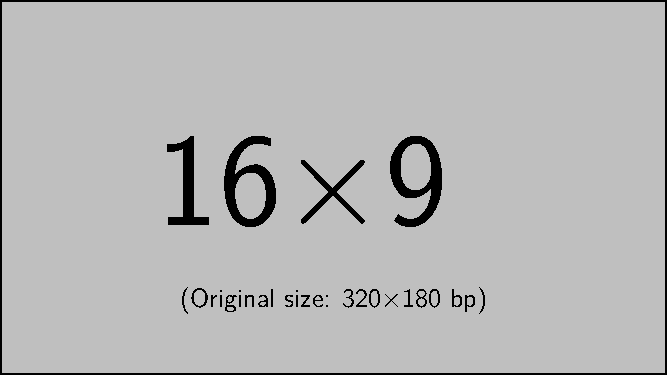
\includegraphics[width=.6\hsize]{figure/example-image-16x9.pdf} \\
   \caption{Example of the figure in two columns.}
\end{figure*}

\subsection{Equations}

Number equations consecutively with equation numbers in parentheses
flush with the right margin, as in (1).  To make your equations more
compact, you may use the solidus ( / ), the exp function, or
appropriate exponents.  Italicize Roman symbols for quantities and
variables, but not Greek symbols.  Use an en dash ( $-$ ) rather than
a hyphen for a minus sign.  Use parentheses to avoid ambiguities in
denominators.  Punctuate equations with commas or periods when they
are part of a sentence, as in

\begin{equation}
 a + b = c.
\end{equation}

Symbols in your equation should be defined before the equation appears
or immediately following.  Use ``(1),'' not ``Eq. (1)'' or ``equation
(1),'' except at the beginning of a sentence: ``Equation (1) is ...''

\subsection{Other Recommendations}

The Roman numerals used to number the section headings are optional.
If you do use them, do not number {\scshape{Acknowledgment}} and
{\scshape{References}}, and begin Subheadings with letters.

Use two spaces after periods (full stops).  Hyphenate complex
modifiers: ``zero-field-cooled magnetization.''  Avoid dangling
participles, such as, ``Using (1), the potential was calculated.''
Write instead, ``The potential was calculated using (1),'' or ``Using
(1), we calculated the potential.''

\bibliography{cites}

\end{document}


%#!platex
%#BIBTEX bibtex manuscript
